\section{Implementation of Algorithms}
\label{sec:imp}
In this section, we discuss the implementation details of our algorithm. Before diving into the details of our implementations, first we look at the architecture of MADlib. Then we discuss the background and implementation details of genetic programming and adaptive boosting.
\subsection{Understanding MADlib architecture}
Performing linear algebra over matrices is at the heart of many statistical methods.And it is quite challenging for relational databases to operate over very large matrices. At a macroscopic scale, the matrices need to be partitioned intelligently so that the partitions can be fit into memory of a single machine and then there should be options for movement of these partitions in and out of database by using SQL constructs. At microscopic level, the database engine needs to be able to invoke efficient linear algebra functions on the data partitions. MADlib uses a number of techniques to address these challenges:

\subsubsection*{User-defined Aggregation}
MADlib uses user-defined aggregates (UDA) as a basic building block in the macroscopic level whenever applicable. UDAs are the natural way in SQL to implement mathematical functions that take arbitrary number of tuples as input. A user-defined aggregate consists of three user-defined functions:
\begin{itemize}
\item A {\it transition function} that takes current transition state and a new tuple and combines them into a new transition state.
\item An optional {\it merge function} that takes two transition states and computes a new combined transition state. This function is only needed for parallel execution.
\item A {\it final function} that takes a transition state and transforms it into output value.
\end{itemize}

However, UDAs are not enough for implementing iterative algorithms which perform multiple passes over the data.

\subsubsection*{Driver functions for Multipass Iteration}
Many statistical and machine learning algorithms are iterative in nature and do multiple passes over the dataset. They cannot be implemented as simple UDAs. MADlib implements complex iterative methods by writing driver user-defined functions (UDF) in Python to control iteration. The driver UDF stores any inter-iteration output into a temporary table and reuses the resulting table in subsequent iterations as needed. Final outputs are also stored in tables unless they are small, and can be queried as needed. As a result all data movement is done inside database engine and its bufferpool.

\subsubsection*{Support for Microprogramming}
MADlib implements row-level UDFs (functions that are called multiple times per row) in C or C++. Thus, these functions can call open source libraries like LAPACK or Eigen. MADlib also includes a sparse matrix library written in C.

\subsubsection*{C++ abstraction layer for UDFs} 
MADlib provides a C++ abstraction layer for making it easier to write driver UDFs. UDFs can be written using standard C++ atomic types as well as vector and matrix types that are native to linear algebra operations. The C++ abstraction layer also provides memory management and exception handling support. Finally, it includes third-party libraries so that developers can write efficient code.

\subsubsection*{Python support for UDFs}
MADlib is still in its early stages of development. So it does not provide a full-fledged Python abstraction layer for writing driver UDFs. It only provides a database access layer via {\ttfamily plpy.py} module. PostrgreSQL PL/Python language currently uses an internal plpy.py module to implement seamless DB access (using classic PyGreSQL interface, pg). The python abstraction layer is still under development.

Currently, most of the MADlib functions require to be cognizant of the schema of the input tables and produce output table with fixed schema. 

\subsection{Genetic Programming for symbolic regression}
\subsubsection{Background}

Genetic programming is a subset of evolutionary algorithms, which is a family of optimization algorithms based on the principle of \textbf{Darwinian natural selection}. As part of natural selection, a given environment has a population of individuals that compete for survival and reproduction. The ability of each individual to achieve these goals determines their chance to have children, in other words to pass on their genes to the next generation of individuals, who for genetic reasons will have an increased chance of doing well, even better, in realizing these two objectives.

~~\\
This principle of continuous improvement over the generations is taken by evolutionary algorithms to optimize solutions to a problem. In the \textbf {initial generation}, a \textbf{population} composed of different \textbf {individuals} is generated randomly or by other methods. An individual is a solution to the problem, more or less good: the quality of the individual in regards to the problem is called \textbf{fitness}, which reflects the adequacy of the solution to the problem to be solved. The higher the fitness of an individual, the higher it is likely to pass some or all of its genotype to the individuals of the next generation.

~~\\
An individual is coded as a \textbf{genotype}, which can have any shape, such as a string (genetic algorithms), a vector of real (evolution strategies) or in our case a tree (genetic programming). Each genotype is transformed into a \textbf{phenotype} when assessing the individual, i.e. when its fitness is calculated. In some cases, the phenotype is identical to the genotype: it is called \textbf{direct coding}. Otherwise, the coding is called indirect. For example, suppose you want to optimize the size of a rectangular parallelepiped defined by its length, height and width. To simplify the example, assume that these three quantities are integers between 0 and 15. We can then describe each of them using a 4-bit binary number. An example of a potential solution may be to genotype 0001 0111 01010. The corresponding phenotype is a parallelepiped of length 1, height 7 and width 10.

~~\\
During the transition from the old to the new generation are called \textbf{variation operators}, whose purpose is to manipulate individuals. There are two distinct types of variation operators:
\begin{itemize}
	\item the \textbf{mutation operators}, which are used to introduce variations within the same individual, as genetic mutations;
	\item the \textbf{crossover operators}, which are used to cross at least two different genotypes, as genetic crosses from breeding.
\end{itemize}

The figure \ref{fig:algorithmes_evolutionnistes_synopsis} summarizes how an evolutionary algorithm works.

\begin{figure}[htb]
	\centering
		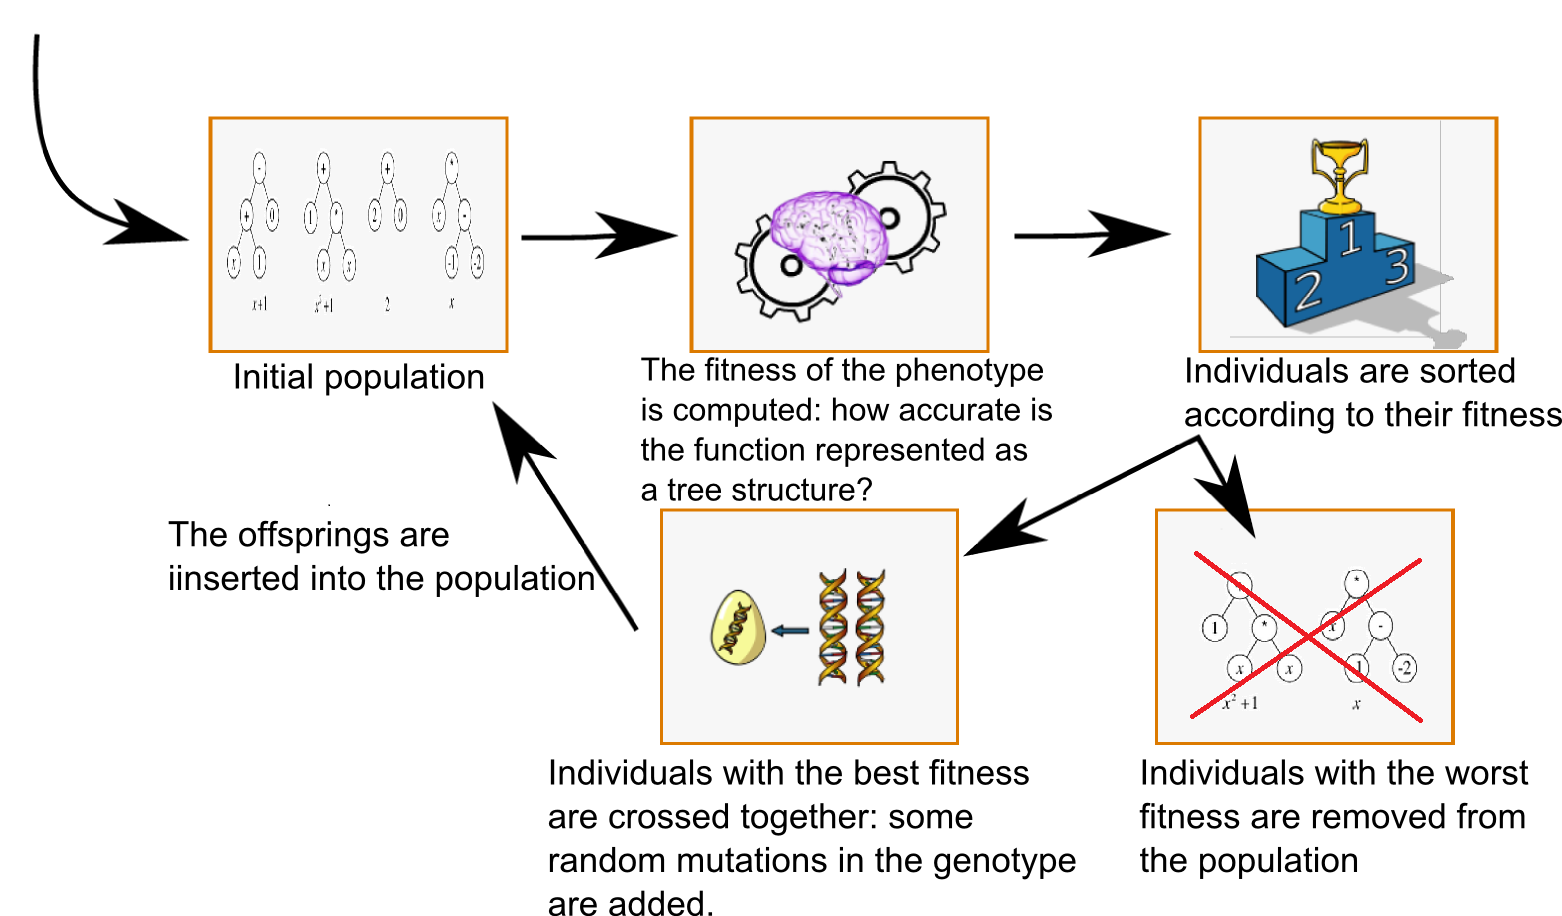
\includegraphics[width=0.8\textwidth]{genetic_programming_regression_synopsis.png}
	\caption[Functioning of an evolutionary algorithm]{Functioning of an evolutionary algorithm: from an initial population of solutions (in symbolic regression, a solution is the tree representing a fraction), they are ranked according to their fitness, the worst ones are eliminated and the best ones are used to produce new solutions.}
	\label{fig:algorithmes_evolutionnistes_synopsis}
\end{figure}

\begin{figure}[htb]
	\centering	
		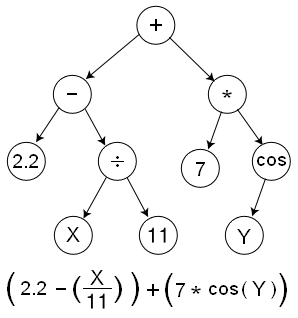
\includegraphics[scale=0.45]{Genetic_Program_Tree.png}
	\caption[A function represented as a tree structure.]{A function represented as a tree structure. Source: Wikipedia}
	\label{fig:Genetic_Program_Tree}
\end{figure}

~~\\
Genetic programming is a perfect suit for symbolic regression. The term "symbolic regression" represents the process during which measured data are fitted by suitable mathematical formula like $x^2 + C$, $sin(x) + 1/e^x$,  etc. The figure \ref{fig:Genetic_Program_Tree} shows how a formula can the represented as a tree. This process is quite well known amongst mathematician and is used when some data of unknown process are obtained. The domain of symbolic regression is of functional nature, i.e. it consists of a function set like ($sin()$, $cos()$, $gamma()$, $MyFunction()$,...) and so called terminal set ($t$, $x$, $p$, ...). The final program is synthesized from a mixture of both sets, and can be quite complicated from a structural point of view. We plan to use genetic programming for symbolic regression in order to unravel unknown relation between some given attributes of a relation. 


\subsubsection{Madlib Implementation}
We implemented the symbolic regression using genetic programming within a Python module for MADlib that depends on the Python evolutionary computation framework DEAP ~\cite{DEAPJMLR2012}. The user can choose whether to store the data in memory, or retrieve by batch: this is a CPU vs. RAM trade-off.

~~\\
Below is an example of a query that runs a symbolic regression, with 100 individuals per population size, 20 generations, and with a maximum size of the trees of 3. It takes 3 attributes as input (x1, x2 and x3) and one attribute as output (y1):

\begin{verbatim}
postgres=# SELECT * from madlib.gp('mock', '{x1, x2, x3}', '{y1}', 100, 20, 3);
\end{verbatim}

\subsection{Adaptive Boosting}
\subsubsection{Background}
Boosting is one of the most important developments in classification methodology. Boosting works by iteratively applying a classification algorithm to re-weighted versions of the training data and then taking a weighted majority vote of the sequence of classifiers thus produced. For many classification algorithms, this simple strategy results in dramatic improvements in performance. While boosting has evolved over the years, we focus on the most commonly used version of boosting known as Adaptive Boosting (AdaBoost) for binary classification developed by Freund and Schapire~\cite{boost96}.

Let us look at a concise description of AdaBoost in a two-class classification setting. We have training data $(x_1, y_1), \ldots, (x_n, y_n)$ with $x_i$ a vector valued feature and $y_i = -1\text{ or }1$. We define $F(x) = \sum_1^M{c_mf_m(x)}$ where each $f_m(x)$ is a classifier producing values $1\text{ or }-1$ and $c_m$ are constants; the corresponding prediction is $\text{sign}(F(x))$. The AdaBoost procedure trains the classifiers $f_m(x)$ on weighted versions of the training sample, giving higher weight to cases that are currently misclassified. This is done for a sequence of weighted samples, and then the final classifier is a linear combination of the classifiers from each stage. The pseudocode for AdaBoost is given in Figure~\ref{fig:adaproc}.

\begin{figure}[ht]
\centering
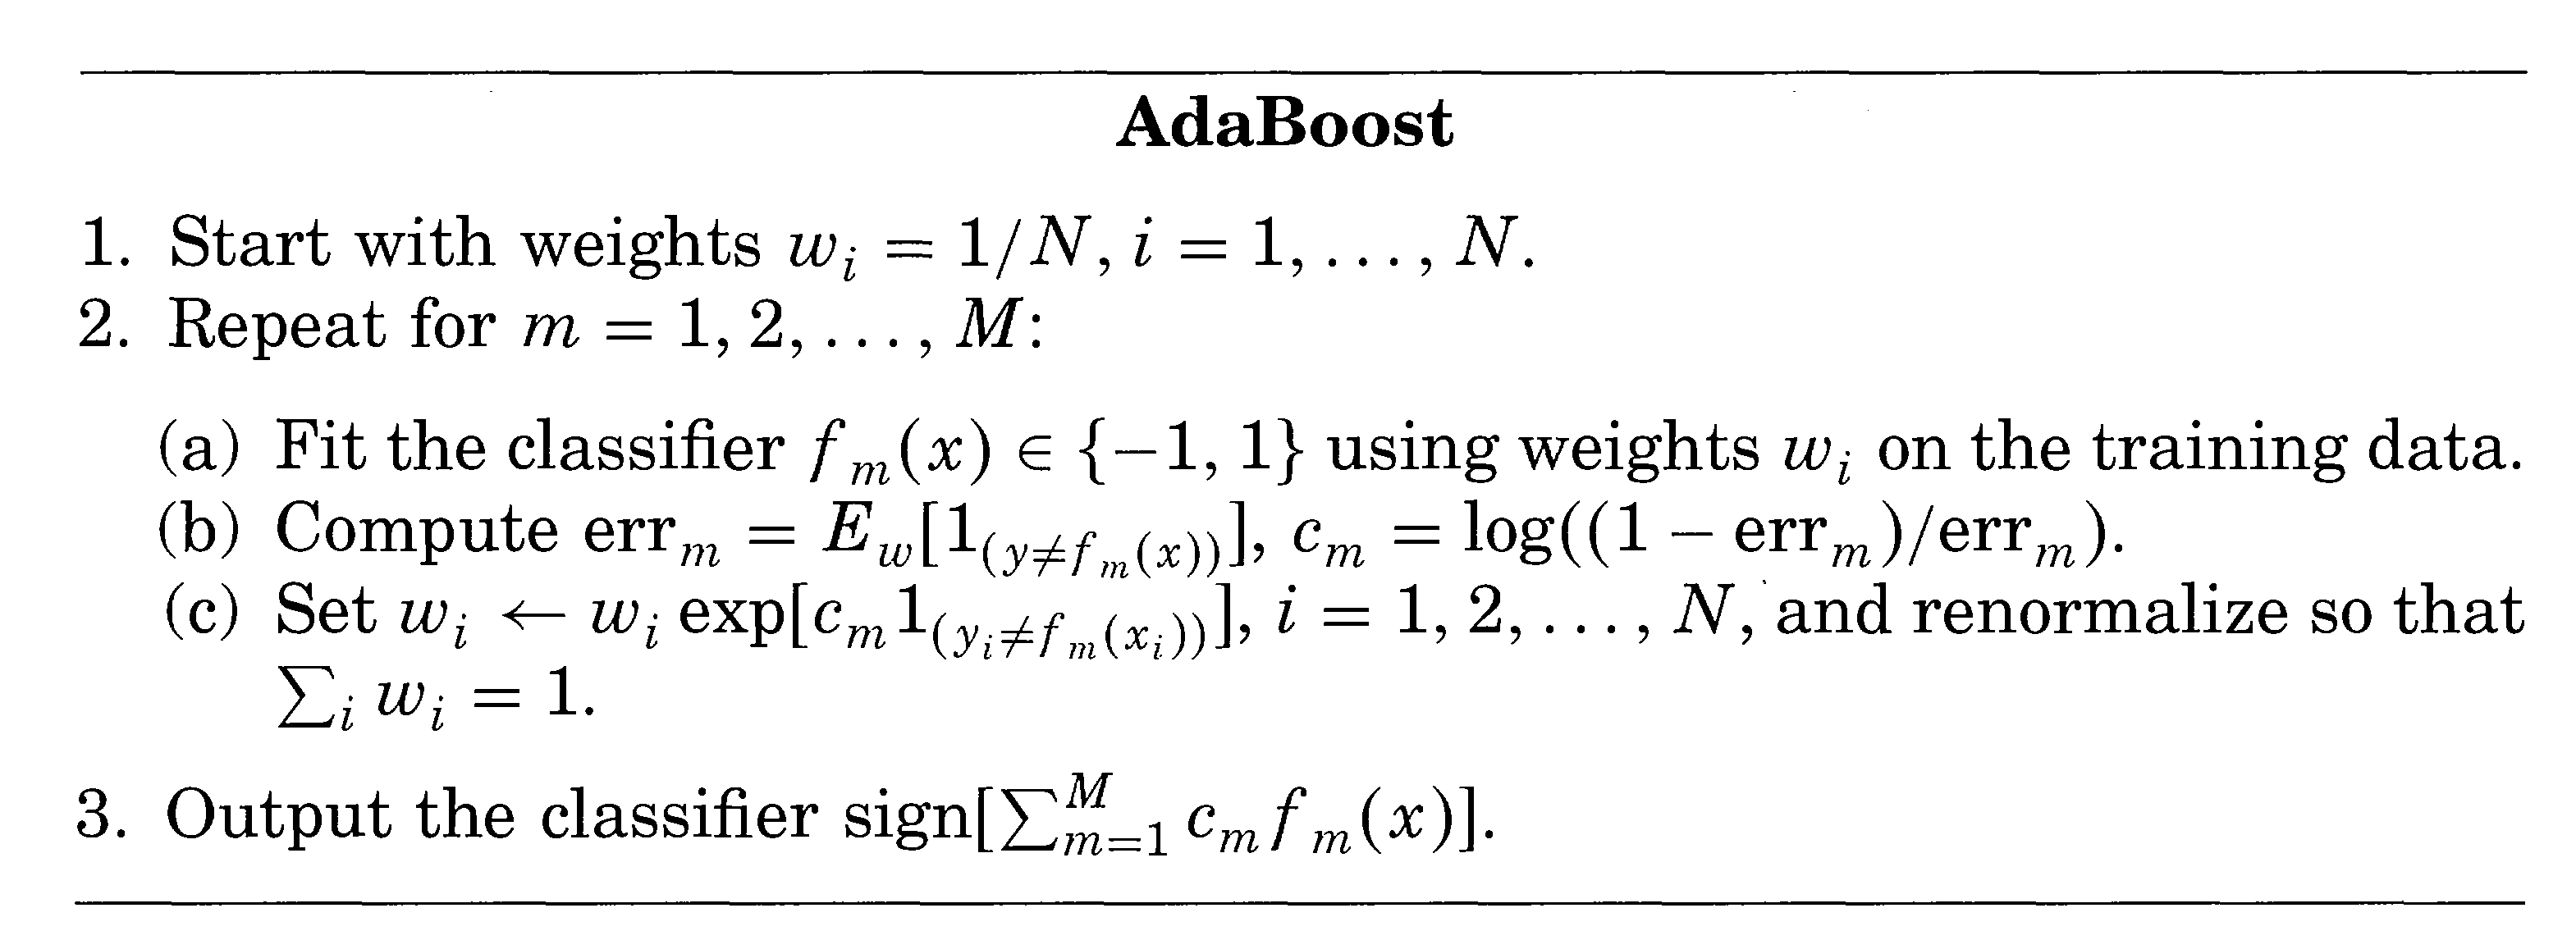
\includegraphics[width=0.8\textwidth]{ada.png}
\caption{AdaBoost algorithm. $E_w$ represents expectation over the training data with weights $w=(w_1,w_2,\ldots,w_N)$ and $I_{(S)}$ is the indicator of the set $S$~\cite{alr00}.}
\label{fig:adaproc}
\end{figure}

We used ``Stumps'' as weak learners. Stumps are single-split trees with only two terminal nodes. Stumps are simple to implement, typically have low variance and success of boosting depends on variance reduction~\cite{alr00}.

\subsubsection{Madlib Implementation}
The challenge in implementing (binary) Adaptive Boosting classification for MADlib is that, the algorithm is iterative in nature and in each iteration, it needs to make a pass over the entire training dataset as well as the weights data. Therefore, it cannot be implemented as a simple user-defined aggregate (UDA). We implemented AdaBoost as a driver UDF in Python. For performing Matrix arithmetic we used the {\ttfamily numpy} package. The control flow of the UDF is shown in Figure~\ref{fig:adaimp}.

\begin{figure}[h]
\centering
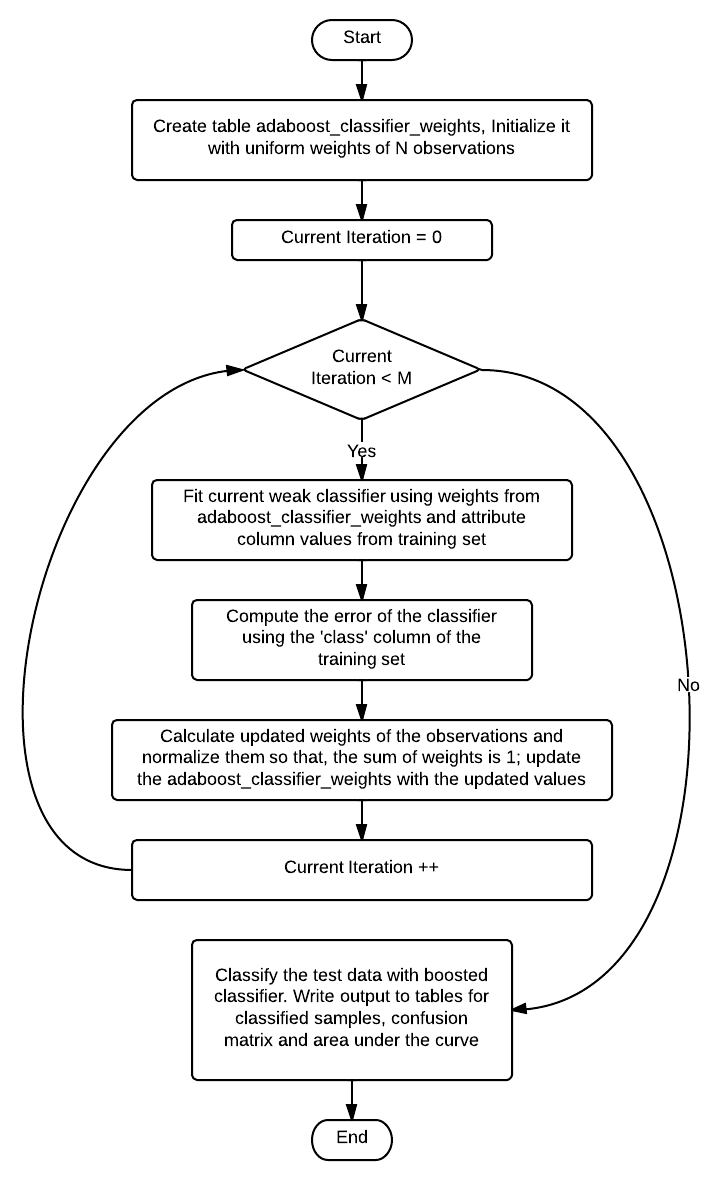
\includegraphics[scale=0.5]{adaimp.png}
\caption{Control Flow of AdaBoost Implementation for MADlib.}
\label{fig:adaimp}
\end{figure}

The row-by-row, batched and in-memory versions differ only in how we access the training and test dataset and weights table. See Appendix E for documentation of usage of AdaBoost module.



